\documentclass{chantbook}

\usepackage[super]{nth}
\usepackage{url}
\usepackage{graphicx}
\usepackage{newpxtext,newpxmath}

\RequirePackage{multicol}
% \chant{cmdName}{Chant Title}
% Defines \cmdName for inserting the chant with a title and \cmdName* for
% inserting it without a title. You can refer to the title itself with
% \cmdName@title. The chant text is set within a chanttext environment you can
% redefine.
\newcommand{\chant}[3]{
  \expandafter\newcommand\csname #1@withtitle\endcsname{%
    \chanttitle{#2}
    \begin{chanttext}
      #3
    \end{chanttext}
  }

  \expandafter\newcommand\csname #1@notitle\endcsname{%
    \ignorespaces#3
  }

  \expandafter\def\csname #1\endcsname{%
    \@ifstar{\csname #1@notitle\endcsname}{\csname #1@withtitle\endcsname}%
  }
}

\chant{paliRefuges}{Pali Refuges}{
  Buddham saranam gacchami\\
  Dhammam saranam gacchami\\
  Sangham saranam gacchami

  Dutiyampi buddham saranam gacchami\\
  Dutiyampi dhammam saranam gacchami\\
  Dutiyampi sangham saranam gacchami

  Tatiyampi buddham saranam gacchami\\
  Tatiyampi dhammam saranam gacchami\\
  Tatiyampi sangham saranam gacchami
}

\chant{sutraOpeningVerse}{Sutra Opening Verse}{
  An unsurpassed, penetrating and perfect dharma is rarely met with even in a
  hundred thousand million kalpas.

  Having it to see and listen to, to remember and accept,\\
  I vow to taste the truth of the Tathagata's words.
}

\chant{fourVows}{Four Vows}{
  Beings are numberless; I vow to save them.\\
  Delusions are inexhaustible; I vow to end them.\\
  Dharma gates are boundless; I vow to enter them.\\
  The Buddha way is unsurpassed; I vow to realize it.
}

\chant{allBuddhas}{All Buddhas}{
  \begin{center}
    All Buddhas, Ten Directions, Three Times \bigspace\largebell\\
    All Honored Ones, Bodhisattvas, Mahasattvas \bigspace\largebell\\
    Wisdom Beyond Wisdom, Maha Prajna Paramita \bigspace\bok
  \end{center}
}

\chant{songOfTheJewelMirrorSamadhi}{Song of the Jewel Mirror Samadhi}{
  The teaching of thusness has been intimately communicated by Buddhas and
  ancestors. Now you have it, so keep it well. Filling a silver bowl with snow,
  hiding a heron in the moonlight, \largebell\ taken as similar they're not the
  same; when you mix them, you know where they are. The meaning is not in the
  words, yet it responds to the inquiring impulse. Move and you are trapped;
  miss and you fall into doubt and vacillation. Turning away and touching are
  both wrong, for it is like a massive fire. Just to depict it in literary form
  is to stain it with defilement. It is bright just at midnight, it doesn't
  appear at dawn. It acts as a guide for beings, its use removes all pains.
  Although it is not fabricated, it is not without speech. It is like facing a
  jewel mirror; form and image behold each other---you are not it, in truth it
  is you. Like a babe in the world, in five aspects complete; it does not go or
  come, nor rise nor stand. ``Baba wawa''---is there anything said or not?
  Ultimately it does not apprehend anything because its speech is not yet
  correct. It is like the six lines of the illumination hexagram: relative and
  ultimate interact---piled up, they make three, the complete transformation
  makes five. It is like the taste of the five-flavored herb, like a diamond
  thunderbolt. Subtly included within the true, inquiry and response come up
  together. Communing with the source, travel the pathways, embrace the
  territory and treasure the road.  Respecting this is fortunate; do not neglect
  it. Naturally real yet inconceivable, it is not within the province of
  delusion or enlightenment. With causal conditions, time and season,
  quiescently it shines bright. In its fineness it fits into spacelessness, in
  its greatness it is utterly beyond location. A hairsbreadth's deviation will
  fail to accord with the proper attunement. Now there are sudden and gradual in
  which teachings and approaches arise. Once basic approaches are distinguished,
  then there are guiding rules.  But even though the basis is reached and the
  approach comprehended, true eternity still flows. Outwardly still while
  inwardly moving, like a tethered colt, a trapped rat---the ancient sages
  pitied them and bestowed upon them the teaching. According to their delusions,
  they called black as white; when erroneous imaginations cease, the acquiescent
  mind realizes itself. If you want to conform to the ancient way, please
  observe the sages of former times. When about to fulfill the way of
  Buddhahood, one gazed at a tree for ten eons. Like a battle-scarred tiger,
  like a horse with shanks gone gray. Because there is the common, there are
  jewel pedestals, fine clothing; because there is the startlingly different,
  there are house cat and cow. Yi with his archer's skill could hit a target at
  a hundred paces. But when arrow-points meet head on, what has this to do with
  the power of skill? When the wooden man begins to sing, the stone woman gets
  up dancing; it's not within reach of feeling or discrimination---how could it
  admit of consideration in thought? Ministers serve their lords, children obey
  their parents; not obeying is not filial and not serving is no help. Practice
  secretly \smallbell\ working within, like a fool, like an idiot \smallbell\ 
  just to continue in this way is called the host within the host.  \bok
}

\chant{ancestorsShort}{Names of the Ancestors (Short)}{
  Bibashi Butsu Daiosho \clank\ Shiki Butsu Daiosho \clank\ Bishafu Butsu
  Daiosho \clank\ Kuruson Butsu Daiosho \clank\ Kunagonmuni Butsu Daiosho
  \clank\ Kasho Butsu Daiosho \clank\ Shakamuni Butsu Daiosho Makakasho Daiosho
  Ananda Daiosho Shonawashu Daiosho Ubakikuta Daiosho Daitaka Daiosho Mishaka
  Daiosho Vashumitsu Daiosho Butsudanandai Daiosho Fudamitta Daiosho Barishiba
  Daiosho Funayasha Daiosho Anabotei Daiosho Kabimare Daiosho Nagyaharajuna
  Daiosho Kanadaiba Daiosho Ragorata Daiosho Sogyanandai Daiosho Kayashata
  Daiosho Kumorata Daiosho Shayata Daiosho Vashubanzu Daiosho Manura Daiosho
  Kakurokuna Daiosho Shishibodai Daiosho Bashashita Daiosho Funyomitta Daiosho
  Hannyatara Daiosho Bodaidaruma Daiosho Taiso Eka Daiosho Kanchi Sosan Daiosho
  Dai-i Doshin Daiosho Daiman Konin Daiosho Daikan Eno Daiosho Seigen Gyoshi
  Daiosho Sekito Kisen Daiosho Yakusan Igen Daiosho Ungan Donjo Daiosho Tozan
  Ryokai Daiosho Ungo Doyo Daiosho Doan Dohi Daiosho Doan Kanchi Daiosho Ryozan
  Enkan Daiosho Taiyo Kyogen Daiosho Toshi Gisei Daiosho Fuyo Dokai Daiosho
  Tanka Shijun Daiosho Choro Seiryo Daiosho Tendo Sokaku Daiosho Seccho Chikan
  Daiosho Tendo Nyojo Daiosho Eihei Dogen Daiosho Koun Ejo Daiosho Tettsu Gikai
  Daiosho Keizan \clank\ Jokin \clank\ Daiosho \bok
}

\chant{femaleAncestors}{Names of the Female Ancestors}{
  Acharya Mahapajapati \clank\  Acharya Mitta \clank\  Acharya Yasodhara \clank\
  Acharya Tissa Acharya Sujata Acharya Sundari-nanda Acharya Vaddhesi Acharya
  Patachara Acharya Visakha Acharya Singalaka-mata Acharya Khema Acharya
  Uppalavanna Acharya Samavati Acharya Uttara Acharya Chanda Acharya Uttama
  Acharya Bhadda Kundalakesa Acharya Nanduttara Acharya Dantika Acharya Sakula
  Acharya Siha Acharya Dhammadinna Acharya Kisagotami Acharya Ubbiri Acharya
  Isidasi Acharya Bhadda Kapilani Acharya Mutta Acharya Sumana Acharya Dhamma
  Acharya Chitta Acharya Anopama Acharya Sukka Acharya Sama Acharya Utpalavarna
  Acharya Shrimala Devi Acharya Congchi Acharya Lingzhao Acharya Moshan Liaoran
  Acharya Liu Tiemo Acharya Miaoxin Acharya Daoshen Acharya Shiji Acharya Zhi'an
  Acharya Huiguang Acharya Kongshi Daoren Acharya Yu Daopo Acharya Huiwen
  Acharya Fadeng Acharya Wenzhao Acharya Miaodao Acharya Zhitong Acharya Zenshin
  Acharya Zenzo Acharya Ezen Acharya Ryonen Acharya Egi Acharya Shogaku Acharya
  Ekan Acharya Shozen Acharya Mokufu Sonin Acharya Myosho Enkan Acharya Ekyu
  Acharya Eshun Acharya Soshin Acharya \clank\  Soitsu Acharya \clank\  Chiyono
  \bok
}

\chant{jiHoSan}{Ji Ho San Shi}{
  \begin{center}
    Ji ho san shi i shi fu \bigspace\largebell\\
    shi son bu sa mo ko sa \bigspace\largebell\\
    mo ko ho ja ho ro mi \bigspace\null\bigspace\null
  \end{center}
  \smallBellRolldown
}

\chant{makaHannyaHaramittaShingyo}{Maka Hannya Haramitta Shingyo}{
  Kan ji zai bo satsu gyo jin han-nya ha ra mi ta ji sho ken go on kai ku do
  is-sai ku yaku sha ri shi shiki fu i ku ku fu i shiki shiki soku ze
  \largebell\ ku ku soku ze shiki ju so gyo shiki yaku bu nyo ze sha ri shi ze
  sho ho ku so fu sho fu metsu fu ku fu jo fu zo fu gen ze ko ku chu mu shiki mu
  ju so gyo shiki mu gen ni bi zes-shin ni mu shiki sho ko mi soku ho mu gen kai
  nai shi mu i shiki kai mu mu myo yaku mu mu myo jin nai shi mu ro shi yaku mu
  ro shi jin mu ku shu metsu do mu chi yaku mu toku i mu sho tok-ko bo dai
  sat-ta e han nya ha ra mit ta ko shin mu kei ge mu kei ge ko mu u ku fu on ri
  is-sai ten do mu so ku gyo ne han san ze sho butsu e han-nya ha ra mit ta ko
  toku a noku ta ra sam myaku sam bo dai ko chi han-nya ha ra mi ta ze dai jin
  shu ze dai myo shu ze mu jo shu ze mu to do shu no jo is-sai ku shin jitsu fu
  ko ko setsu han-nya ha ra mit ta shu soku setsu shu watsu \smallbell\ gya tei
  gya tei ha ra gya tei \smallbell\ hara so gya tei bo ji sowa ka han-nya shin
  gyo \bok
}

\chant{shosaimyoKichijoDharani}{Shosaimyo Kichijo Dharani}{
  \begin{multicols}{2}
    \emph{(3 times)}\\
    No mo san man da\\
    moto nan\\
    oha ra chi koto sha\\
    sono nan to ji to \largebell\bat{1}\\
    en\\
    gya gya\\
    gya ki gya ki\\
    un nun\\
    shifu ra shifu ra\\
    hara shifu ra hara shifu ra\\
    chishu sa chishu sa \smallbell\bat{3}\\
    chishu ri chishu ri\\
    sowa ja sowa ja \smallbell\bat{3}\\
    sen chi gya\\
    shiri ei somo-ko \bok\bat{3}
  \end{multicols}
}

\newcommand{\weDedicateThisMeritTo}[1]{%
  Looking upward we deeply wish for Buddha's true compassion. Bowing down
  we ask the illumination of Buddha's understanding.

  Chanting the #1.

  We dedicate this merit to:

  \smallbell\ $\uparrow$

  Our original ancestor in India, great teacher Shakyamuni Buddha,\\
  Our first female ancestor, great teacher Mahapajapati,\\
  The first ancestor in China, great teacher Bodhidharma,\\
  The first ancestor in Japan, great teacher Eihei Dogen,\\
  Our compassionate founder, great teacher Shogaku Shunryu.

  $\downarrow$ \smallbell

  Gratefully we offer this virtue to all beings $\sim$ \largebell
  \pagebreak[2]
}

\chant{harmonyOfDifferenceAndEquality}{Harmony of Difference and Equality}{
  The mind of the great sage of India is intimately transmitted from west to
  east. While human faculties are sharp or dull, the way has no northern or
  southern ancestors. \largebell\ The spiritual source shines clear in the
  light, the branching streams flow on in the dark. Grasping at things is surely
  delusion, according with sameness is still not enlightenment. All the objects
  of the senses interact and yet do not. Interacting brings involvement,
  otherwise each keeps its place. Sights vary in quality and form, sounds differ
  in pleasing or harsh. Refined and common speech come together in the dark,
  clear and murky phrases are distinguished in the light. The four elements
  return to their natures just as a child turns to its mother.
  \doshidependent{Fire heats, wind moves, water wets, earth is solid, eye and
    sights, ear and sounds, nose and smells, tongue and tastes. Thus with each
    and every thing, depending on these roots the leaves spread forth. Trunk and
    branches share the essence, revered and common each has its speech. In the
    light there is darkness, but don't take it as darkness. In dark there is
    light, but don't see it as light. Light and dark oppose one another like the
    front and back foot in walking. Each of the myriad things has its merit
  expressed according to function and place.} Phenomena exist, box and lid fit,
  principle responds, arrow points meet.  Hearing the words understand the
  meaning; don't set up standards of your own.  If you don't understand the way
  right before you, how will you know the path as you walk? Progress is not a
  matter of far or near, but if you are confused \smallbell\ mountains and
  rivers block your way.  \smallbell\ I respectfully urge you who study the
  mystery; do not pass your days and nights in vain. \bok
}

\chant{ancestorsLong}{Names of the Ancestors (Long)}{
  Bibashi Butsu Daiosho \clank\ Shiki Butsu Daiosho \clank\ Bishafu Butsu
  Daiosho \clank\ Kuruson Butsu Daiosho \clank\ Kunagonmuni Butsu Daiosho
  \clank\ Kasho Butsu Daiosho \clank\ Shakamuni Butsu Daiosho Makakasho Daiosho
  Ananda Daiosho Shonawashu Daiosho Ubakikuta Daiosho Daitaka Daiosho Mishaka
  Daiosho Vashumitsu Daiosho Butsudanandai Daiosho Fudamitta Daiosho Barishiba
  Daiosho Funayasha Daiosho Anabotei Daiosho Kabimare Daiosho Nagyaharajuna
  Daiosho Kanadaiba Daiosho Ragorata Daiosho Sogyanandai Daiosho Kayashata
  Daiosho Kumorata Daiosho Shayata Daiosho Vashubanzu Daiosho Manura Daiosho
  Kakurokuna Daiosho Shishibodai Daiosho Bashashita Daiosho Funyomitta Daiosho
  Hannyatara Daiosho Bodaidaruma Daiosho Taiso Eka Daiosho Kanchi Sosan Daiosho
  Dai-i Doshin Daiosho Daiman Konin Daiosho Daikan Eno Dai\-osho Seigen Gyoshi
  Daiosho Sekito Kisen Daiosho Yakusan Igen Daiosho Ungan Donjo Daiosho Tozan
  Ryokai Daiosho Ungo Doyo Daiosho Doan Dohi Daiosho Doan Kanchi Daiosho Ryozan
  Enkan Daiosho Taiyo Kyogen Daiosho Toshi Gisei Daiosho Fuyo Dokai Daiosho
  Tanka Shijun Daiosho Choro Seiryo Daiosho Tendo Sokaku Daiosho Seccho Chikan
  Daiosho Tendo Nyojo Daiosho Eihei Dogen Daiosho Koun Ejo Daiosho Tettsu Gikai
  Daiosho Keizan Jokin Daiosho

  Gasan Joseki Daiosho Taigen Soshin Daiosho Baizan Mompon Daiosho Jochu Tengin
  Daiosho Shingan Doku Daiosho Senso Esai Daiosho Iyoku Choyu Daiosho Mugai
  Keigon Daiosho Nenshitsu Yokaku Daiosho Sesso Hoseki Daiosho Taiei Zesho
  Daiosho Nampo Gentaku Daiosho Zoden Yoko Daiosho Tenyu Soen Daiosho Ken'an
  Junsa Daiosho Chokoku Koen Daiosho Senshu Donko Daiosho Fuden Gentotsu Daiosho
  Daishun Kan'\-yu Daiosho Tenrin Kanshu Daiosho Sessan Tetsuzen Daiosho Fuzan
  Shunki Daiosho Jissan Mokuin Daiosho Sengan Bonryu Daiosho Daiki Kyokan
  Daiosho Enjo Gikan Daiosho Shoun Hozui Daiosho Shizan Tokuchu Daiosho Nanso
  Shinshu Daiosho Kankai Tokuon Daiosho Kosen Baido Daiosho Gyakushitsu Sojun
  Daiosho Butsumon Sokaku Daiosho Gyokujun So-on \clank\ Daiosho Shogaku \clank\
  Shunryu Daiosho \bok
}

\chant{enmeiJukkuKannonGyo}{Enmei Jukku Kannon Gyo}{
  \begin{multicols}{2}
    \emph{(7$\times$)}\\
    Kan ze on\\
    Na mu butsu\\
    Yo Butsu u in\\
    Yo Butsu u en \largebell\bat{1}\\
    Bup-po so en\\
    Jo raku ga jo \smallbell\bat{7}\\
    Cho nen kan ze on\\
    Bo nen kan ze on\\
    Nen nen ju shin ki \smallbell\bat{7}\\
    Nen nen fu ri shin \largebell\bat{4,5} \bok\bat{7}
  \end{multicols}
}

\chant{lovingKindnessMeditation}{Loving Kindness Meditation Sutra}{
  This is what should be accomplished by the one who is wise, who seeks the
  good, and has obtained peace. \largebell\ Let one be strenuous, upright, and
  sincere, without pride, easily contented, and joyous. Let one not be submerged
  by the things of the world. Let one not take upon oneself the burden of
  riches. Let one's senses be controlled. Let one be wise but not puffed up and
  let one not desire great possessions even for one's family. Let one do nothing
  that is mean or that the wise would reprove. May all beings be happy. May they
  be joyous and live in safety. All living beings, whether weak or strong, in
  high or middle or low realms of existence, small or great, visible or
  invisible, near or far, born or to be born, may all beings be happy. Let no
  one deceive another nor despise any being in any state. Let none by anger or
  hatred wish harm to another. Even as a mother at the risk of her life watches
  over and protects her only child, so with a boundless mind should one cherish
  all living things, suffusing love over the entire world, above, below, and all
  around, without limit. So let one cultivate an infinite good will toward the
  whole world.  Standing or walking, sitting or lying down, during all one's
  waking hours, let one practice the way with gratitude. Not holding to fixed
  views, endowed with insight, freed from sense appetites, one who achieves
  \smallbell\ the way will be freed \smallbell\ from the duality of birth and
  death. \bok
}

\chant{heartOfGreatPerfectWisdomSutra}{Heart of Great Perfect Wisdom Sutra}{
  Avalokiteshvara Bodhisattva, when deeply practicing prajna paramita, clearly
  saw that all five aggregates are empty and thus relieved all suffering.
  Shariputra, form does not differ from emptiness, emptiness does not differ
  from form. \largebell\ Form itself is emptiness, emptiness itself form.
  Sensations, perceptions, formations, and consciousness are also like this.
  Shariputra, all dharmas are marked by emptiness; they neither arise nor cease,
  are neither defiled nor pure, neither increase nor decrease. Therefore, given
  emptiness, there is no form, no sensation, no perception, no formation, no
  consciousness; no eyes, no ears, no nose, no tongue, no body, no mind; no
  sight, no sound, no smell, no taste, no touch, no object of mind; no realm of
  sight\dots\ no realm of mind consciousness. There is neither ignorance nor
  extinction of ignorance\dots\ neither old age and death, nor extinction of old
  age and death; no suffering, no cause, no cessation, no path; no knowledge and
  no attainment.  \doshidependent{With nothing to attain, a bodhisattva relies
  on prajna paramita and thus the mind is without hindrance. Without
  hindrance, there is no fear.  Far beyond all inverted views, one realizes
  nirvana. All buddhas of past, present, and future rely on prajna paramita and
  thereby attain unsurpassed, complete, perfect enlightenment.} Therefore know the
  prajna paramita as the great miraculous mantra, the great bright mantra, the
  supreme mantra, the incomparable mantra, which removes all suffering and is
  true, not false.  Therefore we proclaim the prajna paramita mantra, the mantra
  that says \smallbell\ Gate Gate Paragate \smallbell\ Parasamgate Bodhi Svaha
  \bok
}

\newenvironment{service}{%
  \doshi Perform a standing bow behind the bowing mat and approach the altar.
  Offer one long stick of incense and two pinches of chip incense.

  Step back and bow to the altar, then walk back around to the bowing mat and
  put out your bowing cloth.

  \doan Ring the small bell as the doshi walks around the mat as follows:
  \doshiBowingClothRolldown
  The ringdown ends as the doshi drops the corners of the bowing cloth.
  \doshi Perform nine full bows.
  \doan Ring the large bell once for each bow. The first eight rings are
  followed by muffles as the doshi's hands touch down. The ninth is followed by a
  second ring as the doshi's forehead touches down.
  \firstBows
  \sangha Bow with the doshi.
  \doshi Stand up, leaving the bowing cloth on the cushion.
  \sangha \paliRefuges*
  \doshi Step back and do a standing bow.
  \sangha Switch to shashu.
  \doshi Approach the altar and offer more loose incense. Bow to the altar, then
  return to the bowing mat.
  \doan Ring the large bell once as the doshi bows to the altar, then ring the
  small bell twice as the doshi passes the cushion.
  \takeOutChantBookBells
  \sangha Sit on your cushion.
  \doshi Perform three full bows.
  \doan Ring the large bell for the first two bows, and bok the bell on the
  third.
  \secondBows
}{%
  \par
  \jiHoSan*

  \doan End the ringdown when everyone is ready to bow.
  \doshi Lead the sangha in three bows.
  \doan Ring the small bell for each of the three bows, with a fourth ring as the
  doshi's forehead touches the cushion on the third bow.
  \lastBows

  \doshi Pick up the bowing cloth and wait for the sangha to put away their
  cushions.

  When the sangha is ready, bow behind your cushion.
  \doan Ring the small bell. \bigspace\smallbell
  \tenken Open the zendo doors.
  \doshi Bow again at the zendo threshold.
  \doan Ring the small bell. \bigspace\smallbell
  \doshi Step back and bow again.
  \doan Ring the small bell twice, about two seconds apart.
  \bline{\hfill\smallbell\hfill\smallbell\hfill\null}
  \doan Lead the sangha in a shashu bow.

  Lead the sangha out of the zendo.
}


\begin{document}
% TODO:
% - add instructions for tenken to come to the kokyo's side and when to leave.
% - get the pdfnump or whatever package it is that rearranges pdf pages into
% signatures.
%   - Aim for signatures of 2 folios.
% - prohibit page breaks before \bline
% - make largebell and muffle the same diameter
% - fix page margins
% - clearpage before heart of great perfect wisdom sutra

\frontmatter
\begin{titlepage}
{\Huge\bf Regular Services}
\end{titlepage}

\begin{colophon}
Kannon Do Regular Services Book, Second Printing

\bigskip

\copyright\ 2015, Kannon Do Zen Meditation Center\\
1972 Rock St, Mountain View, CA 94043\\
www.kannondo.org

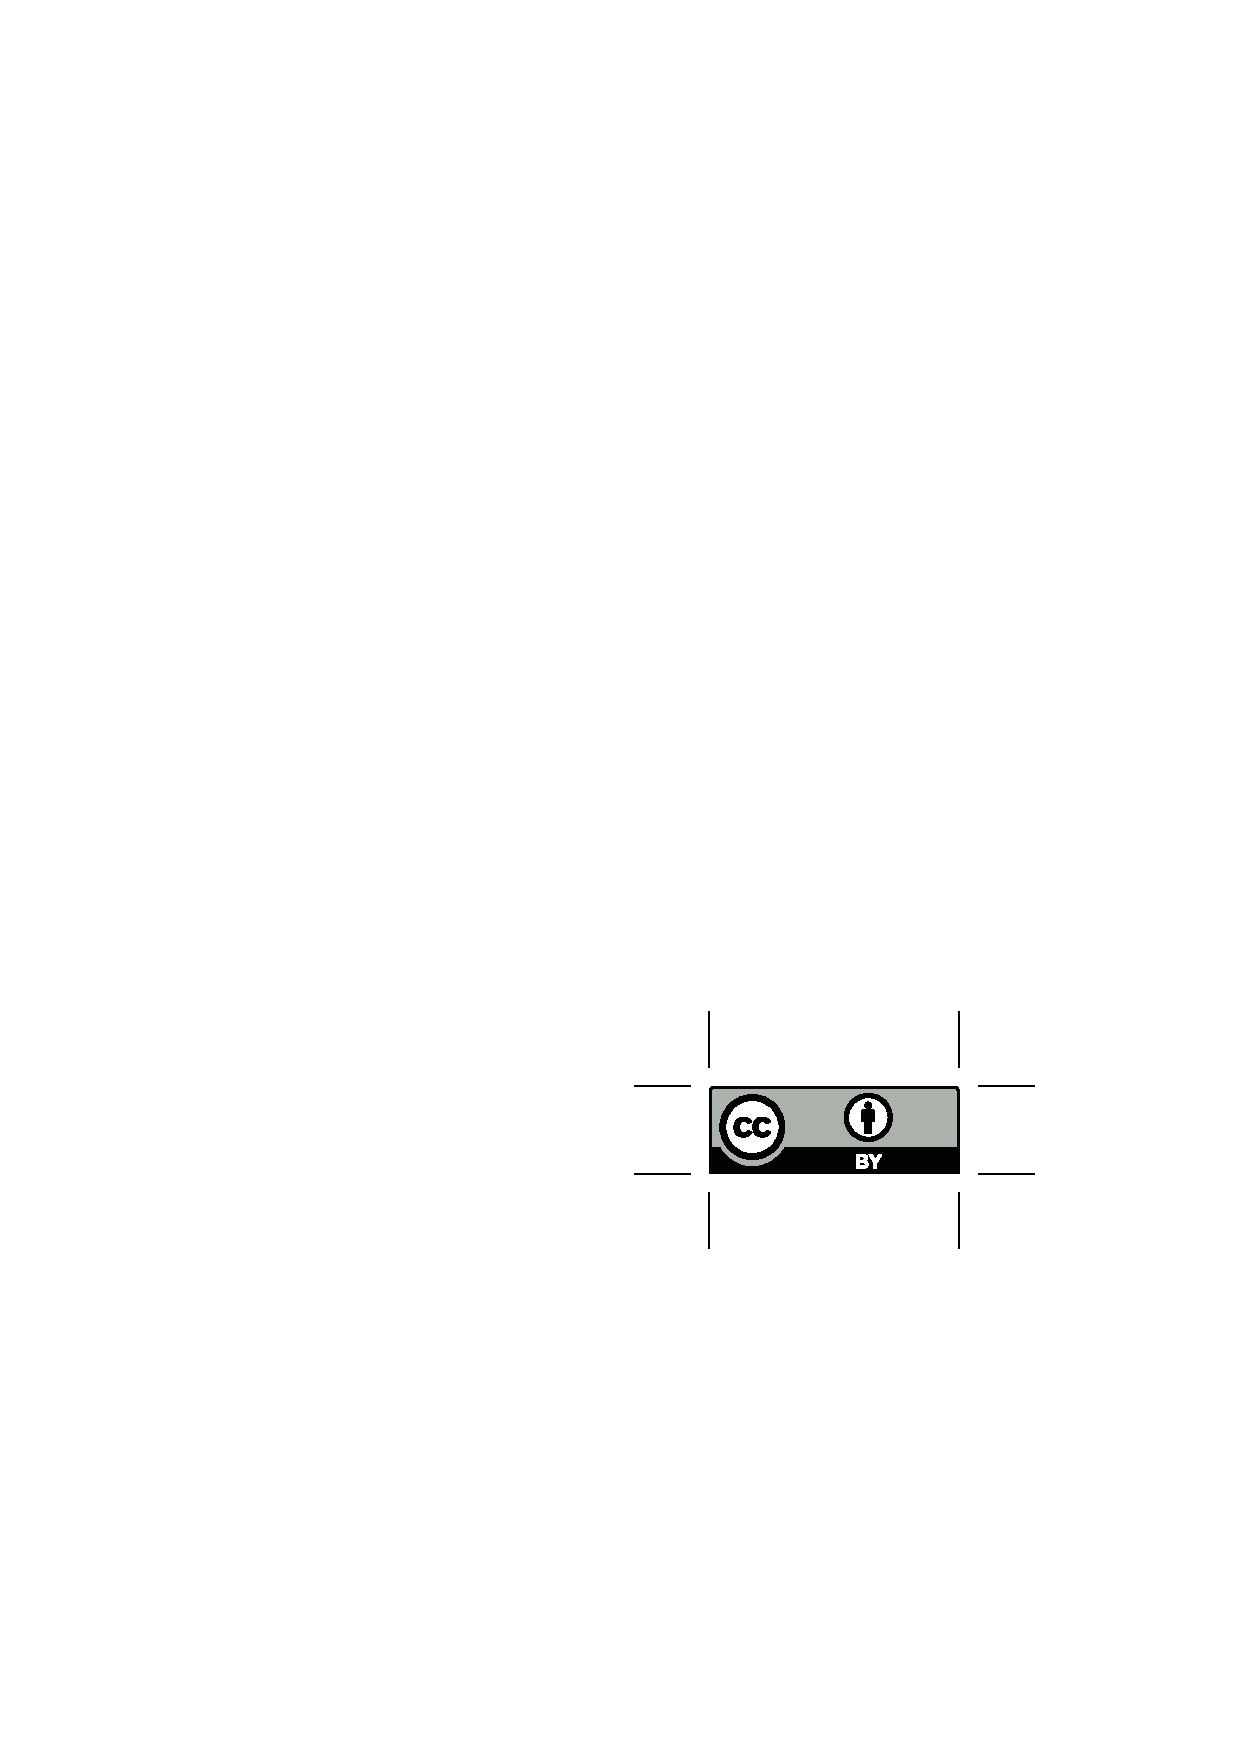
\includegraphics{by}

This work is licensed under the Creative Commons Attribution 4.0 International
License. To view a copy of this license, visit
\url{http://creativecommons.org/licenses/by/4.0/}.

\bigskip

This book was typeset with \LaTeX\ and hand bound at Kannon Do.
\end{colophon}

\begin{dedication}
One thing flows into another\\
and cannot be grasped.\\
Before the rain stops, we hear a bird.

---Shunryu Suzuki
\end{dedication}

\cleardoublepage

\tableofcontents

\mainmatter

\chapter{Introduction}

\section{Service Positions}
\begin{description}
\item[Doshi] An ordained person who leads the service by offering incense and
leading prostrations and bows.
\item[Doan] Rings the bells.
\item[Tenken] Strikes the han (wooden block) to announce Wednesday evening
zazen, minds the lights, and opens the doors.
\item[Kokyo] Leads the chants during service.
\end{description}

\section{Explanation of Symbols}
The different bells are indicated by different symbols.

\subsection{Regular Rings of the Bells}

\begin{tabular}{llc}
Large Bell: & large red circle & \largebell \\
Small Bell: & small red dot & \smallbell \\
Zazen Bell: & small green diamond & \zazenbell
\end{tabular}

In addition to the regular rings, there are four sound effects that can be
produced on the large bell.

\subsection{Effects (\kern-.1ex Always on Large Bell)}
\begin{tabular}{llr}
Muffle: & red circle with $\times$ & \muffle \\
Bok: & red circle with slash & \bok \\
Clank: & red triangle & \clank
\end{tabular}

To produce a \muffle\ \emph{muffle}, hold the playing stick with two hands and hold it
firmly against the top of the bell to stop the ringing. Do not raise the
playing stick until the bell stops ringing. The playing stick should not make a
noise when it meets the top of the bell.

To produce a \bok\ \emph{bok}, hold the playing stick with two hands and bring it
down solidly against the top of the bell, then hold it in place. Do not remove
the playing stick until the bell has stopped ringing.

The difference between a bok and a muffle is whether the playing stick causes
the bell to ring when brought against the bell.

To produce a \clank\ \emph{clank}, grip the playing stick for the \emph{small bell}
like a pencil and bring the tip solidly against the side of the bell, holding
the playing stick against the bell until the bell stops ringing.

\section*{Doshi-Dependent Rings}
The timing of the second and third bell during long chants is determined by the
timing of the doshi's actions, as follows:

\begin{description}
\item[If the doshi goes up to offer incense.] The doshi will stand up and bow.
The doan rings the large bell as he bows. The doshi will go up to the altar and
offer chip incense, then will step back and bow to the altar. The doan rings
the bell as he bows.
\item[If the doshi stays sitting and puts hands in gassho.] Ring the bell as
the doshi's hands come up to gassho, and again as his hands come back down.
\end{description}

If the doshi does nothing, the doan does not ring the bells.

The approximate times to watch for the doshi's actions are indicated by
\doshidependent{blue text in italics.}

\section*{Using the Audio Equipment}
\subsection*{To turn on the audio equipment}
\begin{enumerate}
\item Press the red square button on the audio deck under the table. It will
light up and turn on the whole deck.
\item Bring up the master volume level toggle to the first rectangle.
\item Place the Lavalier next to the doshi's zabuton. Take care that the line
is neatly coiled and tucked under the clip.
\item Pick up the Sony Sound Recorder and turn it. The power button is on the
left side of the recorder. Pull down on the power button for 2 seconds.
\item Uncoil the headphone jacks under the cushions in front of the sound
table. Make sure the headphones are on the table for people to use if needed.
\item Take a seat on the zabuton on the floor next to the mixer. Once the
recorder is one, wait for the doshi to say ``Good evening,'' then hit the
record button. See the instruction sheet, ``Instructions for recording
lectures,'' sitting next to the mixer.
\end{enumerate}

\subsection*{At the end of the lecture}
When the doshi asks if there are any announcements, press the stop button on the
Sony Sound Recorder.

After the doshi concludes the service, open the zendo doors. Start with the
right one (if you are facing the altar) and then the left. Make sure they are
all the way open and the door catch has caught the door. The doshi and tenken
bow together syncronized with the doan bowing with the sangha.

After everyone has left the zendo, turn off the red power button on the mixer,
place the microphones in the bags, and place them below the sound table.

\fontsize{14pt}{16pt}\selectfont

\chapter{Zazen with Jundo}
\section*{At 5:30 AM}

\doan Prepare the altars by lighting the lamps.

Sit in the doan seat facing the bells and wait for the doshi.

\doshi Enter the zendo and perform a standing bow behind the mat. Walk around
the mat to the altar. Offer one long stick of incense, step back, and perform a
standing bow to the altar. Walk back around the bowing mat.

At the bowing mat, place bowing cloth on cushion, and perform three full bows.

\doan Ring the large bell once for each bow:
\jundoBows

\doshi Walk around the room in gassho.

Stand behind your cushion.

(If staying for zazen) put down bowing cloth and stick.

Bow to your cushion, turn and bow to the room, then sit down (or go to dokusan).

\doan Ring the zazen bell three times, evenly spaced, as the doshi bows:
\jundoStartZazen

Turn to face the wall.

\section*{40 minutes later}
\doan Ring the zazen bell once. \bigspace\zazenbell
\sangha Chant the robe chant.

\chapter{Regular Zazen}
\doan Prepare the altars by lighting the lamps.

Sit in the doan seat facing the bells and wait for the beginning of the period
of zazen.

\doan Ring the zazen bell three times, about 2 seconds apart:
\startZazenBells

Turn to face the wall.

\section*{40 minutes later}

\doan Ring the zazen bell once. \bigspace\zazenbell

\chapter{Kinhin}
\doan Ring the zazen bell twice at the end of zazen.
\kinhinBells

Carry the large inkin bell while doing kinhin.

\section*{10 minutes later}

\doan Ring the inkin bell once. \bigspace\zazenbell

\section*{Leaving the zendo}
\doshi Lead the sangha in a standing bow.
\tenken Open the zendo doors.
\doshi Exit the zendo, bowing.

(Outside) bow to the tenken.

\doan Lead the sangha in a shashu bow, synchronized with the doshi's bow to the
tenken.

Lead the sangha out of the zendo.

\chapter{Doan for Sesshin}
\subsection*{Silent Bowing}
\doan Stay seated in the doan seat, facing the bells.
\sangha Take your cushions to the center of the room, as on Saturday.
\doshi Offer incense, then lead the sangha in full bows.
\doan Ring the large bell once for every bow. \bigspace\largebell

At the end of 10 minutes, ring the large bell twice to signify the end of bows.

\bline{\hfill\largebell\hfill\largebell\hfill\null}

The ino or soku will seat everyone for the meal.

\part{Short Service, Wednesday Night}
\thumb{Wed}
\chapter{Wednesday Night}
\section*{At 7:00 PM}
\tenken Begin rolldown.
\doan Enter zendo, turn down overhead lights, light lamps on kaisando and main
altar.
\section*{At 7:10 PM}

\doshi Offer incense at the altar. Walk around bowing mat. Lay out stick,
bowing cloth, and papers. Bow to cushion. Turn and bow to the room. Sit down.

\doan Ring the zazen bell three times, evenly spaced, as the doshi bows.
\jundoStartZazen

\tenken Close the zendo doors and take your seat.

\section*{At 7:50 PM}
\doan Ring the zazen bell one time. \bigspace\zazenbell
\sangha Stand, fluff cushions, bow to cushions, bow to room. Face in to the
room.
\doan Get up and bow with the sangha. Take your seat again after the doshi
bows.
\doshi Lead the sangha in a standing bow.
\tenken Raise the lights.
\doshi Perform a standing bow behind the bowing mat, approach the altar and
offer one long stick of incense and two pinches of chip incense. Step back and
bow to the altar, then walk back around to the bowing mat and put out the
bowing cloth.

\doan Ring the small bell as the doshi walks around the mat as follows:

\doshiBowingClothRolldown

The ringdown ends as the doshi drops the corners of the bowing cloth.

\kokyo Turn to face the altar as the doshi approaches it to offer incense.

\doshi Perform three full bows.

\doan Ring the large bell once for each bow. The first two rings are followed
by muffles as the doshi's hands touch down. The third is followed by a second
ring as his/her forehead touches down.
\firstBows

\sangha Bow with the doshi.

\doshi Approach the altar and offer more loose incense. Bow to the altar.
Return to the bowing mat.

\doan Ring the large bell once as the doshi bows to the altar, then ring the
small bell twice as the doshi passes the cushion.
\takeOutChantBookBells

\sangha Get out your chant books.

\kokyo Retrieve the kokyo's service book and stand to the right of the doan.

\tenken Retrieve the small mokugyo and stand to the right of the kokyo. Play the
mokugyo as the kokyo chants the words of the heart sutra.

\doshi Perform three full bows.

\doan Ring the large bell for the first two bows, and bok the bell on the
third.
\secondBows

\kokyo \heartOfGreatPerfectWisdomSutra

\kokyo May our intention equally extend to every being and place with the true
merit of Buddha's way $\sim$ \largebell

\allBuddhas

\smallBellRolldown

\tenken Replace mokugyo and return to your cushion.
\kokyo Replace the kokyo's service book and return to your cushion.
\doan End the ringdown when everyone has put away their books.
\doshi Lead the sangha in three bows.
\doan Ring the small bell for each of the three bells, with a fourth ring as
the doshi's forehead touches the cushion on the third bow.
\lastBows

\doshi Pick up bowing cloth, stands behind mat. When the sangha is ready,
perform a standing bow toward the altar.

\doan Ring the small bell. \bigspace\smallbell

\doshi Go to your cushion and bow to it.
\doan Ring the small bell. \bigspace\smallbell
\doshi Turn and bows to the room in.
\doan Ring the small bell twice about two seconds apart.
\beSeatedBells
\doshi Invite everyone to be seated.

\section*{Before Lecture}
\sangha Bring your cushions to the middle of the room.
\kokyo Serve speaker water, help with microphone and lectern as necessary,
then return to your seat.

\doshi Come to gassho.
\doan Bok the large bell: \bigspace\bok
\sangha An unsurpassed, penetrating and perfect dharma\\
Is rarely met with even in a hundred thousand million kalpas.\\
Having it to see and listen to, to remember and accept,\\
I vow to taste the truth of the Tathagata's words.

\section*{After Lecture}
\doshi Come to gassho.
\doan Bok the large bell: \bigspace\bok
\sangha Beings are numberless; I vow to save them.\\
Delusions are inexhaustible; I vow to end them.\\
Dharma gates are boundless; I vow to enter them.\\
The Buddha's way is unsurpassed; I vow to realize it.
\sangha Put away your cushions, stand in front of your place.
\doshi Lead everyone in a standing bow.
\tenken Open the zendo doors.
\doshi Exit the zendo, bowing.

(Outside) bow to the tenken.
\doan Lead the sangha in a shashu bow, synchronized with the doshi's bow to
the tenken.

Lead the sangha out of the zendo.

\part{Long Service, First and Third Saturday}
\thumb{\nth{1} \& \nth{3}}
\chapter{Long Service, First and Third Saturday}
\begin{service}
\kokyo \makaHannyaHaramittaShingyo
\kokyo \enmeiJukkuKannonGyo
\kokyo \weDedicateThisMeritTo{Maka Hannya Haramitta Shin Gyo and the Enmei
Jukku Kannon Gyo for protecting life}
\sangha \allBuddhas
\kokyo \songOfTheJewelMirrorSamadhi
\kokyo May we awaken Buddha's compassion and luminous mirror wisdom.

Chanting the Song of the Jewel Mirror Samadhi, we dedicate this merit and
virtue to: \bigspace\clank

\ancestorsShort

\kokyo And to all the great women teachers, known and unknown, remembered
through these names: \bigspace\clank

\femaleAncestors

\kokyo We dedicate our practice to all the great teachers from whom we have
received immeasurable benefit. And we venerate the founder of this temple,
great teacher Shogaku Shunryu. May our life reveal their compassion. Let us
honor their true being $\sim$ \largebell
\end{service}

\part{Long Service, Second and Fifth Saturday}
\thumb{\nth{2} \& \nth{5}}
\chapter{Long Service, Second and Fifth Saturday}

\begin{service}
\kokyo \makaHannyaHaramittaShingyo
\kokyo \shosaimyoKichijoDharani
\kokyo \weDedicateThisMeritTo{Maka Hannya Haramitta Shin Gyo and the Shosaimyo
Kichijo Dharani for removing hindrance}
\sangha \allBuddhas
\kokyo \harmonyOfDifferenceAndEquality
\kokyo May we awaken Buddha's compassion and luminous mirror wisdom. Chanting
the Harmony of Difference and Equality, we dedicate this merit and virtue to:

\ancestorsLong

\kokyo Now we have dedicated our practice to the great teachers who have
transmitted the lamp through four countries. May our life reveal their
compassion. Let us honor their true being $\sim$ \largebell
\end{service}

\part{Service of Well Being, Fourth Saturday}
\thumb{\nth{4}}
\chapter{Service of Well Being, Fourth Saturday}
\begin{service}
\kokyo \makaHannyaHaramittaShingyo
\kokyo \shosaimyoKichijoDharani
\kokyo \weDedicateThisMeritTo{the Maka Hannya Haramitta Shin Gyo and the
Shosaimyo Kichijo Dharani for removing hindrance}
\kokyo \lovingKindnessMeditation
\kokyo \enmeiJukkuKannonGyo
\kokyo May all awakened beings manifest through the three treasures their
luminous mirror wisdom. Having chanted the Loving Kindness Meditation and the
Enmei Jukku Kannon Gyo for protecting life, we dedicate its merit to

The benefit and well being of our great and abiding friends: \hrulefill

And to the benefit of all beings.\\
May they attain Buddha's Way. \largebell
\end{service}
\end{document}
